\section{Faglig vidensgrundlag}


\subsection{Begrebsdefinitioner}

\begin{tabular}{|p{4cm}|p{10cm}|}
\hline
\textbf{ Begreb } & \textbf{Definition} \\
\hline
Brugsmønster & Et brugsmønster viser hvilke scenarier en bruger af et software system kan interagere med \\
\hline
Brugsmønsterdiagram & Et brugsmønsterdiagram er et diagram der viser hvordan forskellige aktører interagerer med forskellige brugsmønstre \\
\hline
Supplerende krav & beskrivelse \\
\hline
MoSCoW & 
MoSCoW er en prioterings model der bruges til at sige hvilke ting man: 
\begin{description}[noitemsep]
    \item [skal] have
    \item [burde] have 
    \item [kan] have
    \item [hvad man ikke] vil have
\end{description}  \\
\hline
 \end{tabular}

 % Teori --------------------------------------------------------------------------------------------------------
\subsection{Teori}
\subsubsection{Udvikling af Brugsmønstermodeller} %-------------------------------
Det første skridt i udviklingen af et brugsmønster er at finde og definere de forskellige aktører der vil interagere med systemet. En aktør kan defineres som alt der kommunikerer med systemet og ikke selv er en del af systemet. Et eksempel på dette kunne være en kunde på en webshop. Disse aktører opstilles i en tabel sammen med de brugsmønstre hver aktør kan tilgå. 
Da kravindsamling er en evolutionær aktivitet, bliver alle aktører ikke nødvendigvis identificeret i første iteration. Det er muligt at identificere primærer aktører i løbet af første iteration, og først senere i forløbet blive i stand til at identificere sekundære aktører, når man får mere viden om systemet. \textit{Primære} aktører interagerer med systemet for at opnå påkrævede systemfunktioner, og ud fra det, få noget ud af at bruge systemet. \textit{Sekundære} aktører støtter systemet så de primærer aktører kan gøre deres arbejde. Når aktørerne er fundet kan brugsmønstrene findes. \textbf{Et brugsmønster angiver et scenarie en aktør kan interagere med}. \\

Når både aktører og brugsmønstre er fundet, kan man opstille et brugsmønster-diagram for at give en visuel forståelse for hvilke aktører der kan tilgå hvilke brugsmønstre. Et eksempel på et brugsmønsterdiagram kan ses nedenfor. \\
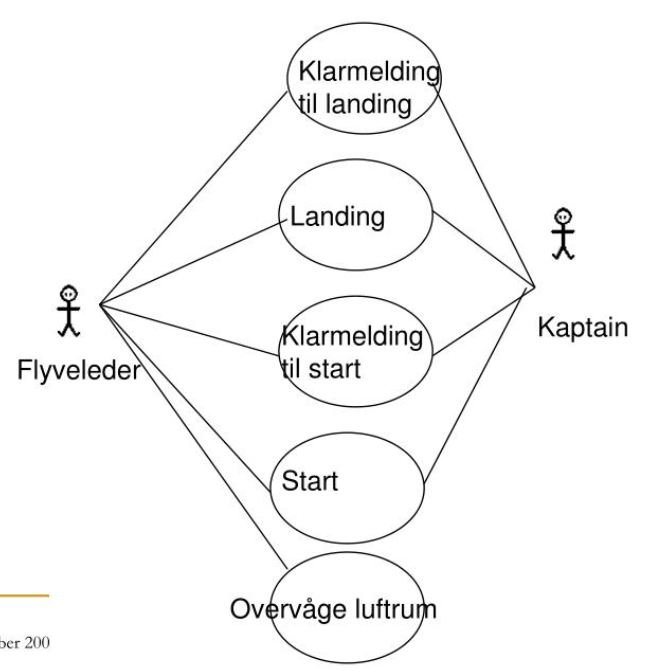
\includegraphics[scale=1]{figures/2. Faglig vidensgrundlag/UseCaseExample.png} \\

Brugsmønstermodellen hjælper udvikleren med at forstå brugeren, så systemet kan konstrueres. Idet der er et samlet billede af hvordan systemet skal se ud, vil udviklingen være mere målfast da kravene og deres forhold til brugeren er klare.

\subsubsection{Supplerende krav} % -------------------------------


\subsubsection{MoSCoW} % ------------------------
MoSCoW er en prioriterings model. Den bruges ofte i software udvikling. 
Modellen i sig selv kan dog bruges, men det anbefaldes at man bruger den sammen med en \textbf{Agile proces}. 
MoSCoW er en vigtig model i software udvikling da, den beskriver hvilken del af softwaren der minimum skal laves før det virker. Der laves en prioritering liste med kunden om hvad de så gerne vil have først.Det bliver så stillet op i en MoSCoW model.

\begin{description}
    \item [Must have] betyder skal have og i software udvikling betyder det, som er minum der skal være med for at softwaren virker. 
    \item [Should have] betyder det som burde være med det kunden rigtig gerne vil have med.
    \item [Could have] betyder det som kunne være med. Hvis der er tid nok. 
    \item [Won't have (this time)] Det som der slet ikke skal prioterres nu, men måske en anden gang. 
\end{description}  \\

% Fagligt Videngrundlag ----------------------------------------------------------------------------
\subsection{Fagligt Vidensgrundlag} \\
Det forventes at læseren for en forståelse for basal programmering i sprogene Java og Python.

\subsubsection{Lovgivningen for visning af krediteringer}
\subsubsubsection{\textbf{Kredit formalia}} \\
Når det kommer til kreditering er der mange regler. Disse regler afhænger bl.a. af hvilken TV-kanal eller land der er tale om. \textbf{I denne opgave vil vi gå ud fra DR's krediteringsregler for TV}. \\

Formålet med krediteringer er at orientere seerne om hvem der har bidraget til et programs tilblivelse. \\

\textbf{1.1 FORM} \\
Målet med krediteringer er at integrere dem så vidt muligt i programmet. Derfor skal kredit altid vises med programrelevant lyd- og billedside.

\textbf{1.2 Varighed} \\
Varigheden af krediteringer afhænger af længden af programmet. Krediteringer for programmer under 60 minutter må maksimalt vare 20 sekunder, hvor programmer der er længere end 60 minutter må have 30 sekunders krediteringer. Større dansk dramatik må have 46 sekunders krediteringer. \\

\textbf{1.3 Hvem skal krediteres} \\
Når det kommer til hvem der skal krediteres, kigges der på medarbejderens eller medvirkenes funktion i programmet. Ifølge ophavsretsloven skal ophavsmænd samt udøvende kunstnere krediteres.
Hver medvirkende har kun ret til én kreditering pr. funktion. Det vil altså sige, at hvis en skuespiller nævnes i starten af programmet, må vedkommende kun nævnes i slutningen hvis vedkommende har andre funktioner.
Hvis flere personer har samme funktion, fremhæves den hovedansvarliges navn grafisk. \\

\textbf{1.4 Eksterne produktioner} \\
Kreditering for eksterne produktioner skal så vidt muligt overholde DR's kreditregler. Indkøbte programmer som spillefilm eller dokumentarer, skal så vidt det forhandlingsmæssigt er muligt, tilpasses DR's kreditregler. Dertil skal der altid være kildeangivelse af producenten. 

\textbf{1.5 Eksterne firmaer og medarbejdere} \\
Når enkelte funktioner bliver udført af personer hos eksterne firmaer (firmaer der ikke er programproducenten), krediteres den enkelte person. I andre tilfælde krediteres det eksterne firma. Eksterne firma samt det eksterne firmas medarbejdere må ikke begge krediteres. \\

\textbf{1.6 Sponsorkreditering} \\
Sponsorer skal krediteres i rulleteksterne, ikke med logo, i slutningen af et program. \\

\textbf{1.7 Citater og arkiv} \\
Ved citater skal ophavsmanden til værket krediteres. Hvis der i citatet er en funktion der indeholder en selvstændigt skabende indsats der har betydning for programmets indhold, skal også denne krediteres. Kilden, fx spillesteder eller andre TV-stationer skal også krediteres. \\
Ved arkivmateriale skal ophavsmanden krediteres. Også her skal der krediteres hvis der i materialet er en funktion der indeholder en selvstændigt skabende indsats, der har betydning for programmets indhold. Nogle programmer kan dog indeholde mange arkivklip, så der skal hertil overvejes om der skal ske en fuld kreditering af alle ophavsmænd. I sådan et tilfælde er det i overensstemmelse med god skik, blot at kreditere i begrænset omfang. \\

\textbf{1.8 Adresser, Konkurrencer MV.} \\
Adresser, vindere af konkurrencer, telefonnr mm. skal vises permanent eller parallelt med almindelig kredit, så dette ikke optager unødvendig tid. \\

\textbf{1.9 Start-kredit} \\
Kredit kan i forbindelse med dramatikprogrammer fordeles mellem start og slut. Her vises funktioner som Instruktør, Manuskript, Oversættelse, Hovedroller mm. i starten af programmet. De øvrige krediteringer vises i slutningen. \\

\subsubsubsection{\textbf{Kredit design}} \\
Også ved design af krediteringer er der regler. Kredit opdeles i to områder. Den nederste tredjedel af skærmen bruges til at vise krediteringer, hvor de øverste to tredjedele bruges til programrelevante billeder. Denne opdeling giver mulighed for at overskrifte det øverste felt og vise programspots der, mens kreditering stadig vises i bunden. \\
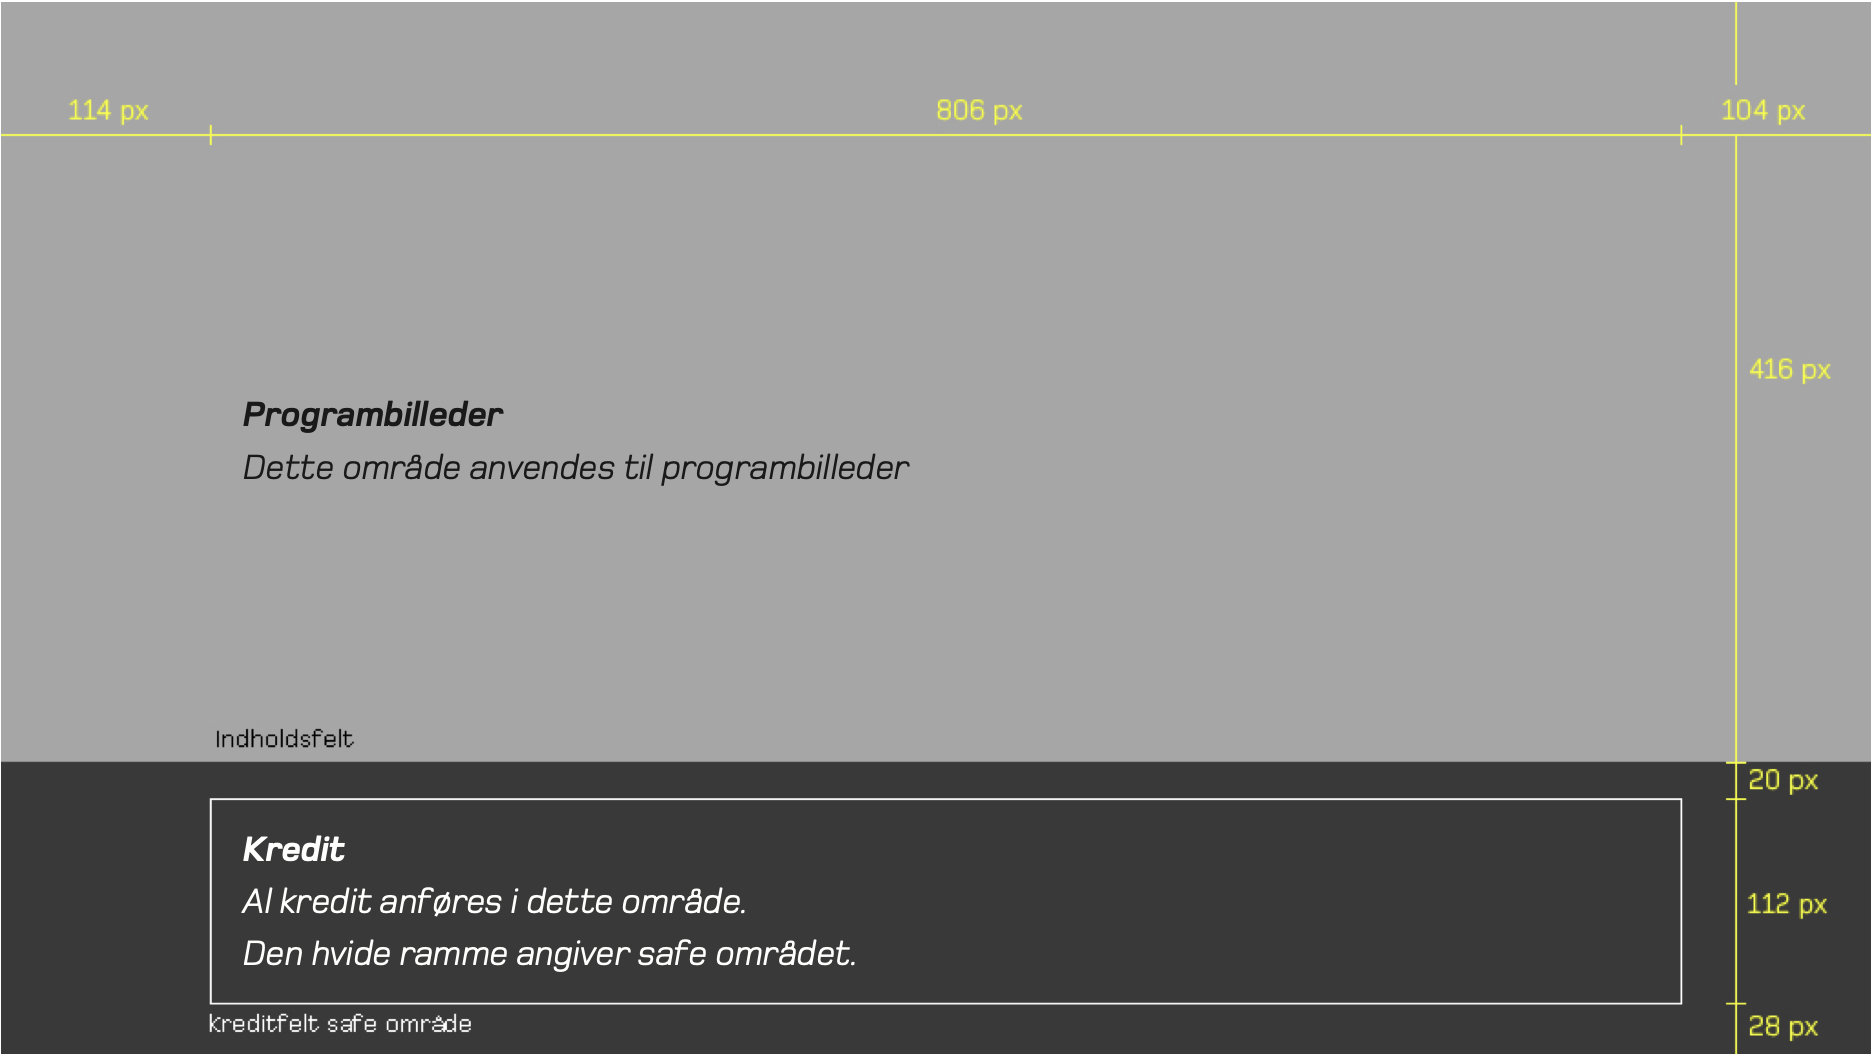
\includegraphics[scale=0.42]{figures/2. Faglig vidensgrundlag/Kredit Design.png}

\subsubsection{TODO: MÅSKE NOGET MED PROGRAMMERING}